\documentclass[11pt,twoside,a4paper]{book}  
% definice dokumentu
\usepackage[czech, english]{babel}
\usepackage[T1]{fontenc} 				% pouzije EC fonty 
\usepackage[utf8]{inputenc} 			% utf8 kódování vstupu 
\usepackage[square, numbers]{natbib}	% sazba pouzite literatury
\usepackage{indentfirst} 				% 1. odstavec jako v cestine, pro práci v aj možno zakomentovat
\usepackage{fancyhdr}					% tisk hlaviček a patiček stránek
\usepackage{nomencl} 					% umožňuje snadno definovat zkratky a jejich seznam

%%%%%%%%%%%%%%%%%%%%%%%%%%%%%%%%%%%%%%%%%%%%%%%%%%%%%%%%%%%%%%%
% informace o práci
\newcommand\WorkTitle{Nástroj pro tvorbu a sdílení HTML5 prezentací na webu}		% název
\newcommand\FirstandFamilyName{Radek Ježdík}															% autor
\newcommand\Supervisor{Ing. Ondřej Macek}															% vedoucí

\newcommand\TypeOfWork{Bakalářská práce}	% typ práce [Diplomová práce | Bakalářská práce | Bachelor's Project | Master's Thesis ]	

% Nastavte následují podle vašeho oboru a programu (pomoc hledejte na http://www.fel.cvut.cz/cz/education/bk/prehled.html)								
\newcommand\StudProgram{Softwarové technologie a management, Bakalářský}	% program
\newcommand\StudBranch{Softwarové inženýrství}           					% obor

%%%%%%%%%%%%%%%%%%%%%%%%%%%%%%%%%%%%%%%%%%%%%%%%%%%%%%%%%%%%%%%
% minimální importy
\usepackage{graphicx}					% pro vkládání obrázků
\usepackage{k336_thesis_macros} 		% specialni makra pro formatovani DP a BP
\usepackage[
pdftitle={\WorkTitle},				% nastaví v informacích o pdf název
pdfauthor={\FirstandFamilyName},	% nastaví v informacích o pdf autora
colorlinks=true,					% před tiskem doporučujeme nastavit na false, aby odkazy a url nebyly šedé při ČB tisku
breaklinks=true,
urlcolor=red,
citecolor=blue,
linkcolor=blue,
unicode=true,
]
{hyperref}								% pro zobrazování "prokliknutelných" linků 

% rozšiřující importy
\usepackage{listings} 			%slouží pro tisk zdrojových kódů se syntax higlighting
\usepackage{algorithmicx} 		%slouží pro zápis algoritmů
\usepackage{algpseudocode} 		%slouží pro výpis pseudokódu

%%%%%%%%%%%%%%%%%%%%%%%%%%%%%%%%%%%%%%%%%%%%%%%%%%%%%%%%%%%%%%%
% příkazy šablony
\makenomenclature								% při překladu zajistí vytvoření pracovního souboru se seznamem zkratek

\let\oldUrl\url									% url adresy budou zobrazeny: <url> 
\renewcommand\url[1]{<\texttt{\oldUrl{#1}}>}

%%%%%%%%%%%%%%%%%%%%%%%%%%%%%%%%%%%%%%%%%%%%%%%%%%%%%%%%%%%%%%%
% vaše vlastní příkazy
\newcommand*{\nomExpl}[2]{#2 (#1)\nomenclature{#1}{#2}} 	% usnadňuje zápis zkratek : Slova ke Zkrácení (SZ)
\newcommand*{\nom}[2]{#1 \nomenclature{#1}{#2}} 			% usnadňuje zápis zkratek : SZ


\usepackage{nameref}


\lstset{
	literate=%
		{á}{{\'a}}1
		{í}{{\'i}}1
		{é}{{\'e}}1
		{ý}{{\'y}}1
		{ú}{{\'u}}1
		{ó}{{\'o}}1
		{ě}{{\v{e}}}1
		{š}{{\v{s}}}1
		{č}{{\v{c}}}1
		{ř}{{\v{r}}}1
		{ž}{{\v{z}}}1
		{ď}{{\v{d}}}1
		{ť}{{\v{t}}}1
		{ň}{{\v{n}}}1
		{ů}{{\r{u}}}1
		{Á}{{\'A}}1
		{Í}{{\'I}}1
		{É}{{\'E}}1
		{Ý}{{\'Y}}1
		{Ú}{{\'U}}1
		{Ó}{{\'O}}1
		{Ě}{{\v{E}}}1
		{Š}{{\v{S}}}1
		{Č}{{\v{C}}}1
		{Ř}{{\v{R}}}1
		{Ž}{{\v{Z}}}1
		{Ď}{{\v{D}}}1
		{Ť}{{\v{T}}}1
		{Ň}{{\v{N}}}1
		{Ů}{{\r{U}}}1
}
\lstset{basicstyle=\ttfamily}

%%%%%%%%%%%%%%%%%%%%%%%%%%%%%%%%%%%%%%%%%%%%%%%%%%%%%%%%%%%%%%%
% vlastní dokument
%%%%%%%%%%%%%%%%%%%%%%%%%%%%%%%%%%%%%%%%%%%%%%%%%%%%%%%%%%%%%%%
\begin{document}
	
	%%%%%%%%%%%%%%%%%%%%%%%%%% 
	% nastavení jazyka, kterým je práce psána
	\selectlanguage{czech}	% podle jazyka práce nastavte na [czech | english]
	\translate				% nastaví české nebo anglické popisy (např. katedra -> department); viz k336_thesis_macros

	%%%%%%%%%%%%%%%%%%%%%%%%%%    
	% Poznamky ke kompletaci prace
	% Nasledujici pasaz uzavrenou v {} ve sve praci samozrejme 
	% zakomentujte nebo odstrante. 
	% Ve vysledne svazane praci bude nahrazena skutecnym 
	% oficialnim zadanim vasi prace.
	{
	\pagenumbering{roman} \cleardoublepage \thispagestyle{empty}
	\chapter*{Zadání projektu}
	Vytvořte nástroj pro tvorbu a sdílení HTML5 prezentací na webu. Webový backend umožní  tvorbu a editaci slidů a jejich sdílení. Pro prezentaci použijte vhodnou JavaScriptovou knihovnu, kterou rozšiřte o možnost testování čtenářů prezentace. Další požadavky na software sesbírejte na základě vytvořeného prototypu.\\\\
	
	\noindent Očekávaný výstup aplikace:
	\begin{enumerate}
		\item Analýza, návrh a implementace webové aplikace pro tvorbu, editaci a sdílení prezentací
		\item Rozšíření prezentační JS knihovny
		\item Nasazení a otestování aplikace
	\end{enumerate}
	\newpage
	}

	%%%%%%%%%%%%%%%%%%%%%%%%%%    
	% Titulni stranka / Title page 
	\coverpagestarts

	%%%%%%%%%%%%%%%%%%%%%%%%%%%    
	% Poděkovani / Acknowledgements 

	\acknowledgements
	\noindent
	Zde můžete napsat své poděkování, pokud chcete a máte komu děkovat.


	%%%%%%%%%%%%%%%%%%%%%%%%%%%   
	% Prohlášení / Declaration 

	\declaration{V~Praze dne 7.\,1.\,2013}
	%\declaration{In Kořenovice nad Bečvárkou on May 15, 2008}


	%%%%%%%%%%%%%%%%%%%%%%%%%%%%    
	% Abstrakt / Abstract 
 
	\abstractpage

	Translation of Czech abstract into English.

	% Prace v cestine musi krome abstraktu v anglictine obsahovat i
	% abstrakt v cestine.
	\vglue60mm

	\noindent{\Huge \textbf{Abstrakt}}
	\vskip 2.75\baselineskip

	\noindent
	Cílem projektu bylo vytvořit webový portál, který bude poskytovat nástroje pro tvorbu a sdílení prezentací postavených na technologiích HTML5. Požadavkem bylo využít potenciálu HTML5 a JavaScriptu ke zvýšení interaktivity prezentace s~uživatelem.

	%%%%%%%%%%%%%%%%%%%%%%%%%%    
	% obsahy a seznamy
	\tableofcontents		% Obsah / Table of Contents 

	% pokud v práci nejsou obrázky nebo tabulky - odstraňte jejich seznam
	\listoffigures			% Obsah / Table of Contents 
	% \listoftables			% Seznam tabulek / List of Tables

	%%%%%%%%%%%%%%%%%%%%%%%%%% 
	% začátek textu  
	\mainbodystarts



\chapter{Úvod}
Tento projekt má za cíl vytvořit webový portál, který uživatelům umožní nejen snadné sdílení prezentací, ale také jejich tvorbu. Prezentace by se měly zaměřovat na podání informací a na případné testování uživatelů z nově nabytých vědomostí. Měly by tak sloužit jak přednášejícím, tak posluchačům či žákům. Pro zobrazení prezentace je využita rodina technologií HTML5 a JavaScriptové knihovny.

\section{Příležitosti}
Od práce na tomto projektu si slibuji větší porozumění technologiím HTML5 a JavaScriptu. Zajímavou příležitostí je tedy vyzkoušení si tvorby webových stránek, které nejsou jen dalším typickým informačním systémem. V tomto projektu lze najít spoustu problémů a nových a zajímavých technologií, na kterých jsem si vyzkoušel vývoj nových klientských aplikací.

\section{Cíle}
Sdílení a tvorba prezentací online není originální myšlenka a v současné době existuje řada známých i méně známých portálů, které dosáhly dobrých výsledků. Proto jsem se rozhodl projekt zaměřit hlavně na použití ve vzdělávacích institucích či školách a nebo na odborných konferencích, kde je důležité v prezentacích podat důležité informace.






\chapter{Analýza}
V této kapitole je čtenář uveden do problematiky HTML prezentací. Dále jsou porovnávány vybrané knihovny, které zajišťují funkčnost HTML prezentací. Nakonec je představena vize vyvíjeného systému a porovnání s podobnými již existujícími systémy.

\section{Popis problému, cíle}
Cílem projektu je vytvořit webový nástroj pro tvorbu, úpravu a sdílení prezentací založených na technologii HTML5.

V současné době se většina aplikací, nástrojů a služeb přesouvá na internet, kde se mimo jiné klade důraz na sdílení mezi uživateli. Prezentace nejsou výjimkou a na trhu lze najít již několik zavedených služeb, které se tvorbou a sdílením prezentací zabývají. S příchodem HTML5 a CSS3\footnote{V době psaní této práce bylo HTML5 ve stádiu návrhu organizací W3C. \url{http://dev.w3.org/html5/decision-policy/html5-2014-plan.html}} se objevily knihovny, které využívají těchto nových technologií pro zobrazení webových prezentací přímo v prohlížeči bez doplňků třetích stran.

\section{HTML5 prezentace}
Prezentace založené na HTML jsou z pohledu kódu běžná webová HTML stránka. K~popisu obsahu snímků se používají sémantické značky běžně používané v HTML (např. nadpisy, odstavce, obrázky). Pro úpravu grafické podoby se používá CSS. K~oživení takovéto stránky a~vytvoření dojmu prezentace a přechodů mezi snímky se používá JavaScript. Funkčnost prezentace tedy zajišťují JavaScriptové knihovny.

Každá z existujících knihoven používá jiná pravidla pro konfiguraci prezentace či jednotlivých snímků. Následující výpis ukazuje zdrojový kód jednoduché HTML prezentace při použití knihovny Deck.js.

\begin{lstlisting}[caption=Ukázka zdrojového kódu HTML prezentace (Deck.js)]
<article class="deck-container">
  <section class="slide">
    <h1>Moje prezentace</h1>
  </section>

  <section class="slide">
    <h2>Nadpis snímku</h2>
    <p>Osnova:</p>
    <ul>
      <li>Bod 1</li>
      <li>Bod 2</li>
      <li>Bod 3</li>
    </ul>
  </section>
</body>
\end{lstlisting}

Zobrazení právě jednoho snímku, přecházení mezi snímky a držení stavu prezentace pak obstarává knihovna samotná. Na autorovi prezentace je jen napsat obsah snímků a dodržet konvence požadované knihovnou.


\section{Výběr JavaScriptové knihovny}
Knihoven pro zobrazení prezentací založených na technologii (X)HTML bylo vytvořena celá řada (viz \cite{htmlslideshowweb}). Většina z nich je ovšem už zastaralá, nefunkční nebo neodpovídající požadovaným kvalitám. Následující seznam uvádí několik zdařilých knihoven, které se objevily po uvedení podpory HTML5 v~prohlížečích.

\begin{itemize}
	\item reveal.js
	\item impress.js
	\item Google I/O HTML5 slide template
	\item deck.js
\end{itemize}


\subsection{Reveal.js} \label{chap:revealjs}
Reveal.js\footnote{\url{https://github.com/hakimel/reveal.js/}} podporuje kromě posunu snímků horizontálně také vnořené snímky, na které se lze dostat posunem dolů. Má několik zajímavých rozšíření, např. podpora syntaxe Markdown pro psaní obsahu a barevné zvýraznění kódu programovacích jazyků pomocí knihovny highlight.js. V novém okně pak umožňuje zobrazit aktuální a následující snímek včetně poznámek přednášejícího.

\subsection{Impress.js}
Impress.js\footnote{\url{https://github.com/bartaz/impress.js/}} se více zaměřuje na vizuální jedinečnost prezentace. Dosahuje toho složitými transformacemi přechodů mezi snímky. Ty jsou rozloženy v~prostoru, a to nejen ve 2D ale i ve 3D, o různých velikostech a při přechodu mezi snímky se pohled působivě otáčí a přesouvá.

Nevýhoda této knihovny je právě v tomto jednoúčelově pojatému zobrazení. Pro účely tohoto projektu je tak knihovna až moc složitá, hlavně kvůli určení pozic snímků a transformací, a pro informativní prezentace se příliš nehodí - přechody mezi snímky spíše vyrušují.

\subsection{Google I/O HTML5 slide template}
HTML5 šablonu od Googlu\footnote{\url{https://code.google.com/p/io-2012-slides/}} používají při svých prezentacích vývojáři na konferencích Google I/O. Knihovna je proto v dobré kvalitě a velmi dobře uzpůsobená pro přednášející. Obsahuje tzv. prezentační mód podobný tomu v reveal.js. Poskytuje také zvýraznění kódu programovacích jazyků a to včetně možnosti zdůraznit jen určitou část kódu, které se přednášející chce věnovat podrobněji.

Knihovna ovšem nenabízí žádnou dokumentaci a tak snižuje možnost na další rozšíření. Dále má prezentace pevnou velikost a tak na menších displejích či oknech jsou snímky oříznuté. Nevýhodou je také o něco složitější konfigurace.

\subsection{Deck.js}
Knihovna deck.js\footnote{\url{https://github.com/imakewebthings/deck.js}} je v základu o něco jednodušší než knihovny výše. Je napsaná v jQuery, je velmi dobře zdokumentovaná a rozšiřitelná. Existuje pro ni řada pluginů, například již zmíněný prezentační mód či podpora Markdown syntaxe pro popis snímků.

\subsection{Zhodnocení}
Pro účely tohoto projektu byla použita knihovna deck.js, která je o něco jednodušší. Líbí se mi více celkový vzhled a jednoduchost a to, že je postavena na jQuery. Případně lze také využít existujících rozšíření nebo vytvořit vlastní. Reveal.js ovšem urazil během práce na tomto projektu velký kus cesty a v současné době je asi nejvíce rozšířenou a používanou knihovnou pro HTML prezentace.


\section{Webový portál}
Pro uživatele má portál sloužit jako prostředník pro sdílení prezentací – ať už v~rámci portálu mezi jeho uživateli nebo
posíláním URL odkazů na prezentace v~emailech, příspěvcích na sociálních sítích Facebook nebo Twitter a dalších. V principu se tak bude podobat portálům jako YouTube, SlideShare nebo GitHub, které se zaměřují na vystavení vlastní tvorby (videí, prezentací, kódu) a její sdílení.

Sdílení prostřednictvím webového portálu je dvojího typu. Uživatelé mohou sledovat jiné uživatele a o aktivitách těchto sledovaných uživatelů, například publikace nové prezentace, bude snadněji upozorněn. Druhý typ je pak sdílení opačným směrem, od autora prezentace uživatelům portálu. Uživatele si autor vybere podle uživatelského jména či e-mailu.

Důležitá je také zpětná vazba od uživatelů prohlížející si prezentace. Řešením je možnost uživatelů přidávat komentáře k jednotlivým prezentacím.

\section{Editor}
Důležitou částí tohoto projektu je editor pro úpravy prezentace. Protože obsah prezentace je tvořen pomocí HTML, nabízí se
několik možností, jak editaci pojmout:

\begin{enumerate}
	\item psaním samotného HTML kódu.
	\item využitím editoru WYSIWYG (What You See Is What You Get).
	\item využitím jednoduchého textového značkovacího jazyka (lightweight markup language).
\end{enumerate}

Psaní samotného HTML kódu bylo vyloučeno bez většího váhání. HTML není nijak úsporný značkovací jazyk a pro uživatele, kteří neznají HTML, by byl překážkou. Na druhou stranu ale poskytuje největší možnou kontrolu nad podobou a funkčností prezentace. Kdyby ovšem editor měl být založen pouze na psaní HTML kódu, nebyl by vůbec potřeba - pro většinu uživatelů by pak bylo výhodnější použít nástroje, na které jsou zvyklí, a pak pouze nahrát hotovou prezentaci na web.

Editor WYSIWYG je koncept dobře známý z desktopových aplikací. Jedná se o přímou úpravu obsahu a uživatel nepřichází do styku se zdrojovým kódem. Jeho největší výhodou je pak jednoduchost pro uživatele, kteří výsledek svých úprav vidí okamžitě. Ve webovém prostředí se používá pro jednoduché vytváření stránek, například v CMS systémech. Nevýhodou je, že neexistuje standard, který by dodržovaly všechny prohlížeče. Poskytuje také menší kontrolu nad výsledným kódem. 

Vybrána byla nakonec poslední možnost - jednoduchý textový značkovací jazyk, jímž se bude popisovat obsah snímku. Zdrojový text se následně převádí do kódu HTML. Více je popsáno v~kapitole \ref{chap:realizace} \nameref{chap:realizace} na str. \pageref{chap:realizace}.

\section{Prohlížení prezentace}
Zajímavou vlastností, která se liší od ostatních webových služeb pro prohlížení prezentací, byla možnost poskytnout větší interaktivitu s uživatelem. Protože je prezentace běžná HTML stránka, lze využít možností webových technologií pro vytvoření nových vlastností prezentace.

Jednou z nich je možnost odpovídat na otázky a kontrolovat správné odpovědi přímo v prezentaci. Uživatelé si pak mohou vyzkoušet, co se z prezentace naučili. Navíc je možné zobrazit doplňkový text při správné či špatné odpovědi. Ten pak může obsahovat nejen vysvětlení správné odpovědi, ale třeba i odkaz na snímek týkající se dané otázky.

\section{Rešerše existujících řešení}
Během analýzy byly také vyhledány a vyzkoušeny již existující služby, jejichž funkčnost se nejvíce podobá zadání tohoto projektu. Následující odstavce popisují jejich funkci a rozdíly.

\subsection{SlideShare}
SlideShare\footnote{\url{http://www.slideshare.net}} je na internetu velmi známý webový portál pro sdílení prezentací. Obsahuje podobné mechanismy sdílení a zpětné vazby a umožňuje prezentace umisťovat na jiné stránky (tzv. embedded presentace). Prezentace jsou ovšem velmi statické – bez animací a bez větší interaktivity s~uživatelem. Některé prezentace jsou jen obrázkové, nejde tedy označit text ani následovat odkaz. Největší nevýhodou je, že prezentace nelze na portálu přímo tvořit, lze je pouze nahrávat ve formátech PDF, PPT a dalších z~lokálního úložiště. Jakákoliv změna v~prezentaci se tak musí nahrát znovu.

\subsection{Prezi}
Prezi\footnote{\url{http://www.prezi.com}} funguje na podobném principu jako SlideShare, ale zaměřuje se daleko více na grafickou stránku a zakládá si na kreativitě uživatelů a vyjádření jejich idejí pomocí celkového vzhledu prezentace. Prezentace se značně liší od běžných prezentací, které známe například z~Microsoft PowerPoint. Jejich použití se hodí hlavně pro vyjádření nějaké myšlenky či vize, méně se hodí pro podání důležitých informací. Pro zobrazení prezentace používá technologii Flash.

\subsection{Rvl.io}
Rvl.io\footnote{\url{http://www.rvl.io}} je služba od autora knihovny reveal.js popsané na str. \pageref{chap:revealjs}, kterou také používá pro zobrazení prezentací. Služba umožňuje sdílení i tvorbu prezentací přímo na webu. Sdílení je založeno na předávání adresy URL, poskytuje ale také vkládání prezentace do jiných stránek, podobně jako SlideShare. Pro úpravu prezentací využívá WYSIWYG editor, který ale poskytuje jen nezbytné minimum funkcí. Tento portál je velmi mladý a uveden byl po měsíci od započetí práce na tomto projektu. Služba byla v~době psaní této práce stále ve fázi beta testování.




\chapter{Návrh}

\section{Funkční požadavky}
Následující odstavce popisují uživatelské role, které figurují v systému, a jaké tyto role mají možnosti využití systému či práva.\\\\

\noindent \textbf{Nepřihlášený uživatel} bude mít možnost:
\begin{itemize}
	\item \textbf{prohlížet veřejně dostupné prezentace}, k~tomu použije 
		\begin{itemize}
			\item vyhledávací formulář na webu.
			\item adresu URL na stránku s prezentací, kterou dostane jiným komunikačním kanálem.
		\end{itemize}
	\item \textbf{vyhledat prezentace} vyhledávacím formulářem podle názvu nebo autora, aby mohl
		\begin{itemize}
			\item zhlédnout hledanou prezentaci.
			\item číst komentáře pod prezentací.
			\item zobrazit prezentace hledaného uživatele.
		\end{itemize}
	\item \textbf{přihlásit se} do systému pomocí přihlašovacího formuláře, aby získal oprávnění přihlášeného uživatele (viz níže).
	\item \textbf{registrovat se} do systému pomocí registračního formuláře, aby se mohl přihlásit.
\end{itemize}


\noindent \textbf{Přihlášený uživatel} bude mít možnost:
\begin{itemize}
	\item \textbf{vytvářet} prezentace pomocí editoru prezentací.
	\item \textbf{posílat komentáře} k~prezentacím, ke kterým má přístup, pomocí formuláře pod prezentací.
	\item \textbf{prohlížet veřejné a jemu sdílené} prezentace.
	\item \textbf{vyhledat prezentace} vyhledávacím formulářem podle názvu nebo autora, aby kromě toho co může nepřihlášený uživatel:
		\begin{itemize}
		\item \textbf{sledovat nebo zrušit sledování} hledaného uživatele.
		\end{itemize}
	\item \textbf{vidět seznam jemu sdílených prezentací}.
	\item \textbf{vidět seznam veřejných prezentací} uživatelů, které \textbf{sleduje}.
	\item \textbf{odhlásit se}.
\end{itemize}


\noindent \textbf{Autor prezentace} bude mít možnost:
\begin{itemize}
	\item \textbf{upravit prezentaci} v~editoru, aby ji o něco doplnil nebo ji opravil
	\item \textbf{smazat prezentaci}
	\item \textbf{smazat jakýkoliv komentář} k~vlastní prezentaci
	\item \textbf{sdílet prezentaci} ostatním uživatelům portálu
\end{itemize}


\noindent \textbf{Autor komentáře} bude mít možnost:
\begin{itemize}
	\item smazat svůj komentář
\end{itemize}


\section{Nefunkční požadavky}
\begin{itemize}
	\item Systém bude přístupný přes webové rozhraní
	\item Systém bude pro uživatele nezávislý na platformě
	\item Systém bude využívat technologii HTML5
	\item Pro prezentace bude systém využívat JavaScriptovou knihovnu
\end{itemize}



\section{Doménový model}
\begin{figure}[ht]
	\begin{center}
		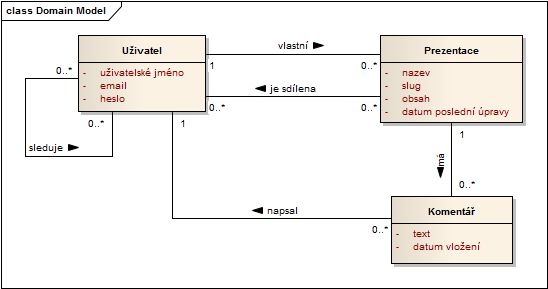
\includegraphics[width=14cm]{PRO-img/PRO-img001.png}
		\caption{Diagram doménového modelu}
		\label{fig:domainModel}
	\end{center}
\end{figure}

\subsection{Uživatel}
Registrovaný a přihlášený uživatel má výhody oproti nepřihlášenému (viz výše).

Pro úspěšnou registraci uživatele do systému musí nepřihlášený uživatel zadat:

\begin{itemize}
	\item \textbf{uživatelské jméno}, pod kterým se bude prezentovat a přihlašovat. Stejné uživatelské jméno musí být v systému registrováno jenom jednou
	\item \textbf{e-mail}, který nebude zveřejněn a bude sloužit pro aktivaci účtu a případně bude informačním kanálem (notifikace, změna hesla, apod.)
	\item \textbf{heslo}, které bude chránit jeho účet (min. 4 znaky)
\end{itemize}
Uživatelé se mohou navzájem sledovat. Uživatel je pak snadněji upozorněn na nové prezentace od sledovaných uživatelů.

\subsection{Prezentace}
Prezentace představuje jednu prezentaci, kterou uživatel pomocí systému vytvořil (je jejím autorem). Má tyto povinné
vlastnosti:

\begin{itemize}
	\item \textbf{název}, pod kterým se daná prezentace bude zobrazovat ve výpisech, a s tím související:
	\item \textbf{slug} - zjednodušený název (malá písmena anglické abecedy, čísla a pomlčky), pod kterým bude prezentace dostupná přes adresu URL
	\item \textbf{obsah}, jenž představuje složitější objekt textů jednotlivých snímků a různých nastavení prezentace
\end{itemize}
Prezentace může být sdílena ostatním uživatelům portálu.

\subsection{Komentář}
Komentář je uživatelem napsaná poznámka k nějaké prezentaci. Komentář může vkládat každý přihlášený uživatel. Povinnými
vlastnostmi jsou:

\begin{itemize}
	\item \textbf{text komentáře} – obsah zprávy
	\item \textbf{datum a čas}, kdy byl komentář vložen
\end{itemize}
Komentář se váže k~jedné prezentaci a jednomu uživateli (autorovi komentáře).



\section{Serverová část}
Webový back-end jsem se rozhodl napsat v~PHP s~použitím českého frameworku Nette \footnote{\url{http://nette.org/}}, s kterým mám dobré zkušenosti. Nette framework mi ušetřil spoustu času, protože všechny důležité funkce, které bych jinak musel řešit a ladit vlastními silami, zvládá elegantně již v~základu. Jeho použití je jednoduché a přímočaré a navíc je velmi dobře otestovaný (mnoha uživateli i vlastními testy). Pro uchování dat byla použita databáze MySQL.


\section{Klientská část}
Front-end je pak poháněn JavaScriptem s~frameworkem jQuery. Pro vzhled a grafické uživatelské rozhraní byl použit framework Bootstrap, který velmi usnadnil prototypování portálu bez nutnosti tvořit a ladit vlastní vzhled. Výhodou je i to, že Bootstrap poskytuje responsivní design a tak by se měl web chovat a zobrazovat dobře i na mobilních zařízeních.

Pro zobrazení prezentací byla použita již zmíněná knihovna deck.js.


\section{Editor}
Editoru jsem přikládal větší význam, a proto používá pár technologií navíc. Jako nejdůležitější se ukázalo použití JavaScriptového MVC frameworku AngularJS\footnote{\url{http://angularjs.org/}}. Jeho hlavní předností je dvoucestné provázání dat mezi pohledem (view) a modelem. Každá změna v~modelu se automaticky propaguje do pohledu a naopak. Snižuje se tak množství kódu, který otrocky nastavuje nebo zobrazuje data při jednotlivé změně.

Pro panel nástrojů, který uživateli ulehčí práci se zdrojovým~textem ve formátu~Texy!\footnote{\url{http://texy.info/}}, byla použita knihovna Texyla\footnote{\url{https://github.com/janmarek/Texyla}}.



\chapter{Realizace} \label{chap:realizace}
V~první fázi vývoje se počítalo s~použitím WYSIWYG editoru pro úpravu snímků. Existuje mnoho knihoven, které WYSIVYG
editor různě implementují. Protože ale neexistuje žádný standard pro přímou editaci kódu HTML, každý prohlížeč se chová
trochu jinak a zároveň každá knihovna si různé věci implementuje po svém.

Nejdříve jsem zkoušel použít pro editaci zdrojového HTML kódu prezentace knihovnu Aloha Editor. Kromě potíží se
zobrazením panelu nástrojů byla největším problémem licence (pozn.: nedávno byla licence změněna na GPLv2).

Přešel jsem tedy na editor Mercury, který se zdál být vhodnější a komplexnější. I když je to JavaScriptová knihovna,
byla vyvíjena v~Ruby pro použití v~Rails aplikacích a tak bylo hodně věcí přizpůsobeno těmto technologiím (například
počítala s~partial pohledy, které se posílají AJAXem ze serveru). Nicméně knihovna není na jazyce Ruby závislá a lze ji
použít bez něj.

Zde se ale po chvíli objevily problémy technického rázu – prohlížeče se právě díky neexistujícímu
standardu chovaly rozdílně nebo se nechovaly podle očekávání. Výsledkem pak byl například špatný HTML kód nebo kód,
který se už nedal nijak pomocí editoru opravit ani smazat. Jedním z~největších problémů bylo vkládání nového řádku.
Prohlížeč někdy vložil značku odřádkování {\textless}br{\textgreater} někdy nový odstavec {\textless}p{\textgreater}.
Chování tak nebylo předvídatelné. Objevily se i další chyby/bugy v~použitelnosti, na které jsem se pak snažil
upozornit\footnote{viz \url{https://github.com/jejacks0n/mercury/issues/253}} autora knihovny. Chyba dosud nebyla opravena.

Všechny tyto problémy nakonec vyústily k rozhodnutí použít značkovací jazyk, tzv. Lightweight markup language, který
převádí text do HTML. V~poslední době získávají tyto jazyky velkou popularitu kvůli jednoduchosti a velmi dobré podobě
výsledného HTML kódu. Asi nejvíce používaný takovýto jazyk je, hlavně ve světě IT, Markdown, který byl původně napsán v
Perl. Vzniklo mnoho portů této knihovny do různých jazyků, včetně PHP. Port pro PHP je ovšem velmi komplexní a zdálo se
mi nemožné ho upravit pro potřeby implementace jistých funkcí do prezentace.

Rozhodl jsem se proto použít jazyk Texy!, který je Markdownu podobný, ovšem syntaxe se občas liší. Texy! je velmi dobře
rozdělené na moduly a jednotlivé konverze se provádějí pomocí callbacků zaregistrovaných podle regulárních výrazů.

Největší výhodou byla ovšem možnost specifikovat CSS třídy nebo určit zarovnání textu či obrázku. To je něco, co Markdown neumí. Velkou výhodou Texy! je také velmi dobrá podpora typografie. Například sekvenci znaků „\lstinline|+-|“ nahradí za jediný znak „$\pm$“, jednoduchou pomlčku nahrazuje za spojovník (pokud je to ve větě potřeba), tři tečky nahradí za jediný znak trojtečky nebo vkládá nedělitelné mezery za spojky atp. Při použití v~prezentacích jsem si to dokázal představit jako dobrý bonus.


\section{Rozložení editoru}
Pro rozložení editoru jsem se inspiroval u běžných nástrojů pro tvorbu prezentací (Microsoft PowerPoint, OpenOffice
Impress) a rozdělil na obrazovku na náhled všech snímků po levé straně obrazovky a na editaci právě upravovaného snímku
vpravo. Protože používám značkovací jazyk namísto přímé editace HTML kódu, bylo nutné dále rozdělit tuto část na
textové pole, do kterého se bude psát text ve značkovacím jazyce, a na velký náhled snímku po konverzi do HTML kódu.
Textové pole má navíc panel nástrojů, který dokáže vkládat značky (například nadpis, nebo kurzívu) pomocí tlačítek.

\begin{figure}[ht]
	\begin{center}
		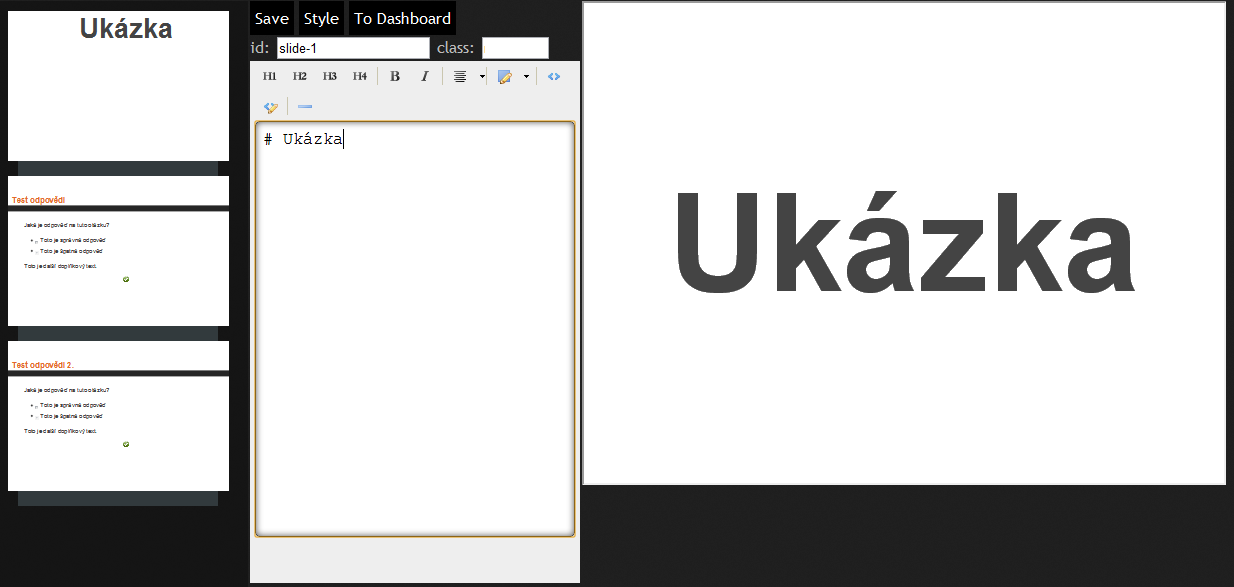
\includegraphics[width=14cm]{PRO-img/editor.png}
		\caption{Ukázka rozložení editoru}
		\label{fig:editorLayout}
	\end{center}
\end{figure}

Toto rozložení se ukázalo jako ne zcela dobré. Vzhled editoru je nyní postaven na velmi jednoduchém CSS a neladí se
stylem zbytku webu, protože po přidání Bootstrap frameworku, který mimo jiné upravuje globální styly prvků, vypadají
náhledy jinak než ve skutečnosti. Dalším problémem jsou jisté technologické nedostatky jako například zmenšování obsahu
snímku pro přizpůsobení výšce a šířce náhledu. Proto se bude editor zjednodušovat, aby na obrazovce bylo co nejméně
rušivých elementů a dodržoval stejný vzhled jako zbytek webu.


\section[Chování editoru]{Chování editoru}
Ze serveru se nejdřív získá celá prezentace jako JavaScriptový objekt. HTML kód každého snímku se pak vloží do panelu
s~malými náhledy. Malý náhled snímku je pomocí CSS pravidla zmenšen, protože jinak by obsah byl stejně velký jako
v~normálním zobrazení prezentace. Po kliknutí na malý náhled se objeví v~textovém poli pro úpravu snímku zdrojový text
v jazyce~Texy! a ve velkém náhledu vpravo se objeví kompletní snímek s~inicializovanou knihovnou deck.js včetně funkční
interakce.

Změna textu snímku se automaticky posílá na server a po zkonvertování se kód HTML vrací v~odpovědi. Následně se
aktualizují oba náhledy. Aby se na server neposílala každá úprava snímku (např. po napsání každého písmene), byla
implementovaná čekací doba 1 sekundy. Pokud po změně snímku uplyne tato doba, během které nebyla provedena žádná další
úprava, pošle se požadavek na server.


\section{Úprava Texy! syntaxe}

\subsection{Markdown syntaxe}
Protože je jazyk Markdown tak rozšířený, chtěl jsem syntaxi Texy! pro psaní snímků co nejvíce přiblížit syntaxi
Markdownu.

Syntaxe Texy! je Markdownu velmi podobná. Jeden z~nejvíce patrných rozdílů byl v~syntaxi nadpisů. Proto jsem konvertor
upravil a změny otestoval pomocí jednotkových testů.

\begin{lstlisting}[caption=Ukázka syntaxe]
## Nadpis snímku

Odstavec s **tučným** textem a *kurzívou*.

- seznam
  - s vnořenými odrážkami
\end{lstlisting}

\subsection{Nová syntaxe}
Zároveň bylo potřeba upravit konvertor a implementovat vlastní pravidla konverze textu do HTML. Tato úprava se týkala
možnosti uživatele odpovídat na otázky během prohlížení prezentace. Jedna se pak může vyskytovat na jednom snímku.

Bylo potřeba vymyslet a implementovat syntaxi na vložení zaškrtávacího pole, které by uživatel zaškrtl jako správnou
odpověď na otázku položenou na snímku.

Syntaxe byla zvolena takto:

\begin{lstlisting}[caption=Syntaxe odpovědí]
[+] pro vložení zaškrtávacího pole ke správné odpovědi
[-] pro vložení zaškrtávacího pole ke špatné odpovědi
\end{lstlisting}

Pro vyhodnocení správnosti odpovědí se při konverzi automaticky vkládá vyhodnocovací tlačítko na konec snímku. Po jeho
stisku uživatelem se kontroluje, že pole u správných odpovědí jsou zaškrtnutá a u špatných odpovědí nikoli. Správnost
či nesprávnost je pak zvýrazněna CSS třídou u každého pole.

U snímků s~otázkou lze také vložit i doplňkový text, který se zobrazí při správné resp. špatné odpovědi. Autor
prezentace tak může uvést bližší informace k~odpovědi na danou otázku nebo odkázat na jiný snímek prezentace či jinou
stránku.

Pro vložení takového bloku textu byla použita podobná syntaxe jako pro ostatní účelové bloky textu v~syntaxi Texy!
(např. blok kódu). Použití syntaxe je následující:

\begin{lstlisting}[caption=Syntaxe doplňkových textů]
/--correct
Tento text se zobrazí při **správné** odpovědi
\--

/--incorrect
Tento text se zobrazí při **špatné** odpovědi
\--
\end{lstlisting}



\chapter{Nasazení}

\section{Server}
Pro chod systému je nutný spuštěný webový server, na kterém běží PHP a databáze MySQL. Pro vývoj používám hotové řešení WAMP (Windows, Apache, MySQL, PHP) jménem EasyPHP. Verze komponent:

\begin{itemize}
	\item Apache 2.2
	\item PHP 5.3
	\item MySQL 5.5
\end{itemize}

Pro nasazení na produkční prostředí jsem se rozhodl využít cloudového systému PHP Fog\footnote{\url{http://phpfog.com}}. Pro malý počet aplikací a malý rozsah poskytuje své služby zdarma. V placených řešení je pak největší výhodou možnost škálování instancí aplikace či paměti nebo velké množství rozšíření (např. analytické nástroje či optimalizační nástroje pro databázi). Server uchovává aplikaci jako git repozitář a tak pro nahrání nové verze aplikace stačí příkaz push.

V listopadu 2012 bylo ovšem oznámeno ukončení provozu PHP Fogu a postupné odpojování bezplatných aplikací v průběhu prosince. Jako náhrada byla doporučena podobná služba AppFog\footnote{\url{http://www.appfog.com/}} od stejné firmy.



\chapter{Shrnutí}
Projekt byl velmi zajímavý. Vyzkoušel jsem si několik nových technologií, zejména AngularJS, který určitě budu dál sledovat a snad s~ním i někdy znovu pracovat. Opět jsem ale došel k~závěru, že zkoumání a použití nových a neznámých vlastností v~technologiích HTML(5) není jednoduché a bezproblémové.

Jsem rád, že jsem použil Nette framework, který dobře znám a tak jsem neměl tolik problémů u~serverové části. Ze začátku jsem se ovšem rozhodoval, jestli si nevyzkoušet nějakou jinou technologii, například dnes moderní Ruby on Rails nebo Node.js. Mohu ale říct, že bych si nepřál znovu dělat tento projekt v~jiné technologii, neboť by mi to přineslo o to více problémů.

Více práce by si rozhodně zasloužila podoba editoru a obecná uživatelská přívětivost. Jinak ale výsledek projektu hodnotím kladně.

\bibliography{BP-ref}{}
\bibliographystyle{unsrt}

\end{document}

















